\documentclass[../TG_magistrsko_delo_sections.tex]{subfiles}
\graphicspath{{\subfix{../images/}}}

\begin{document}
V tem poglavju bomo pokazali, da lahko v vsakem ciklu, ki vsebuje vsaj dve točki, poiščemo Štefanovo zaporedje, razen če vsaka točka v ciklu menja stran. Dokaz bomo izvedli tako, da bomo konstruirali zaporedje in na koncu preverili, da gre za Štefanovo zaporedje.
\begin{trditev}\label{lem:stef-ne-menja}
Cikel, ki vsebuje vsaj dve točki, vsebuje Štefanovo zaporedje, če vsaj ena točka ne menja strani.
\end{trditev}
\begin{proof}
Naj bo $m$ naravno število večje ali enako $2$ in naj bo $\mathcal{O}$ cikel sestavljen iz $m$ različnih točk. Naj bo množica $\mathcal{M}$ največji tak $\mathcal{O}$-interval, ki vsebuje točki $p, q$ in take točke iz cikla $\mathcal{O}$, ki menjajo strani. Množica $\mathcal{M}$ ne vsebuje nobene točke, ki ne menja strani. To pomeni, da za poljubno točko $x \in \mathcal{M} \cap \mathcal{O}$ vse točke iz množice $\mathcal{O}_x$ menjajo strani. Pri konstrukciji Štefanovega zaporedja si bomo pomagali z množico $\mathcal{S} \subseteq \mathcal{O}$, ki vsebuje vse točke, ki so kandidati za nekončne člene Štefanovega zaporedja. V množici $\mathcal{S}$ ležijo take točke $x \in \mathcal{O} \cap \mathcal{M}$, ki jih funkcija $f$ slika dlje od točke $c$ kot katerokoli drugo točko iz množice $\mathcal{O}_x$ (slika~\ref{fig:S}). 
\begin{figure}[h]
  \centering
  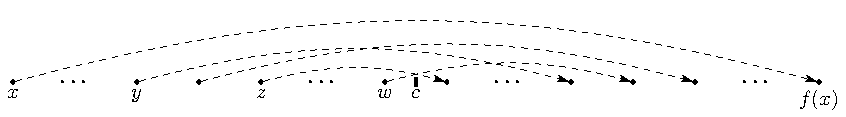
\includegraphics{mnozica_S.pdf}
% \caption[caption za v kazalo]{Dolg caption pod sliko}
  \caption[Konstrukcija množice S.]{Točka $x$ pripada množici $\mathcal{S}$, medtem ko točka $y$ pripada množici $\mathcal{M}$ ne pa tudi množici $\mathcal{S}$, saj se točka $z$ slika bolj stran od točke $c$ kot točka $y$.}
  \label{fig:S}
\end{figure}
Za vsak $x \in \mathcal{O} \cap \mathcal{M}$ velja, da je $x$ iz množice $\mathcal{S}$, če je $\mathcal{O}_{f(w)} \subseteq \mathcal{O}_{f(x)}$ za vsako točko $w \in \mathcal{O}_x$. Množica $\mathcal{S}$ zagotovo ni prazna množica, saj vsebuje točki $p$ in $q$. Sedaj lahko definiramo preslikavo $\sigma : \mathcal{S} \to \mathcal{O}$, ki slika element Štefanovega zaporedja v naslednji člen tega zaporedja. Za $\sigma(x)$ vedno izberemo točko iz množice $\mathcal{O}_{f(x)}$. Točka $x$ je vsebovana v množici $\mathcal{S}$, torej menja strani. To zagotavlja, da točki $x$ in $\sigma(x)$ ležita na nasprotnih straneh točke $c$. Točko $\sigma(x)$ določimo na naslednji način:
\begin{enumerate}[label={(\arabic*)}]
\item\label{def:sigma1} Če $f(x) \in \mathcal{M}$, potem je $\sigma(x)$ tista točke iz množice $\mathcal{O}_{f(x)}$, ki se s funkcijo $f$ slika najdlje od centra $c$. Velja vsebovanost:
$$f(\mathcal{O}_{f(x)}) \subseteq \mathcal{O}_{f(\sigma(x))}.$$
\item\label{def:sigma2} Če $f(x) \notin \mathcal{M}$, potem za $\sigma(x)$ izberemo katero koli točko iz $\mathcal{O}_{f(x)}$, ki ne menja strani.
\end{enumerate}
Iz definicije preslikave $\sigma$ vidimo, da v primeru~\ref{def:sigma1} točka $\sigma(x)$ leži v množici $\mathcal{S}$, saj menja strani in se slika bolj stran od točke $c$ kot katero koli drugo število iz množice $\mathcal{O}_{\sigma(x)}$. Primer si lahko pogledamo na sliki~\ref{fig:sigma}.
\begin{figure}[h]
  \centering
  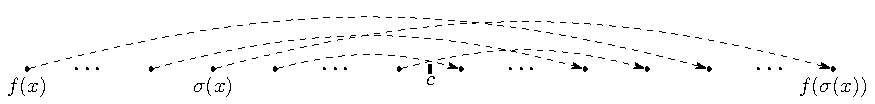
\includegraphics{sigma.pdf}
% \caption[caption za v kazalo]{Dolg caption pod sliko}
  \caption{Ker $f(x)$ menja strani, smo točko $\sigma(x)$ določili po primeru~\ref{def:sigma1}.}
  \label{fig:sigma}
\end{figure}

V primeru~\ref{def:sigma2} $\sigma(x)$ ne leži v množici $\mathcal{S}$, saj ne menja strani. Glede na to, da so v množici $\mathcal{S}$ kandidati za nekončne člene zaporedja, je $\sigma(x)$, ki ga dobimo v primeru~\ref{def:sigma2}, dober kandidat za končen člen zaporedja.

Števili $x$ in $\sigma(x)$ ležita na nasprotnih straneh točke $c$. Če je število $\sigma^2(x)$ dobro definirano, tudi števili $\sigma(x)$ in $\sigma^2(x)$ ležita na nasprotnih straneh točke $c$, kar pomeni, da točki $x$ in $\sigma^2(x)$ ležita na isti strani točke $c$. Kot smo utemeljili v poglavju~\ref{stefan_zap}, je za dokaz zelo pomembno, da se točke spiralno oddaljujejo od točke $c$, kot kaže slika~\ref{fig:spiral} in je podrobneje opisano v definiciji Štefanovega zaporedja v točkah~\ref{eq:š2} in~\ref{eq:š3}. Za vsako točko $x$ iz štefanovega zaporedja bi radi videli, da je $\sigma^2(x)$, če ta obstaja, bolj stran od točke $c$ kot točka $x$. Torej, $\sigma^2(x) \notin \mathcal{O}_x$.


\begin{lema}\label{lem:vtms}
Če obstaja taka točka $x \in \mathcal{S}$, za katero je $\sigma^2(x) \in \mathcal{O}_x$, potem vse točke cikla $\mathcal{O}$ menjajo stran.
\end{lema}
\begin{proof}
Denimo, da je za neko točko $x \in \mathcal{O}$ točka $\sigma^2(x)$ dobro definirana in da je vsebovana v množici $\mathcal{O}_x$. Potem so dobro definirane vse točke $x, y:=\sigma(x)$ in $z:=\sigma(y) = \sigma^2(x)$. Da lahko izračunamo $\sigma(x)$ ali $\sigma(y)$, morata točki $x$ in $y$ ležati v množici $\mathcal{S}$. Točka $y=\sigma(x)$ je izračunana po pravilu~\ref{def:sigma1} v definiciji preslikave $\sigma$, iz česar lahko sklepamo, da velja vsebovanost:
$$f(\mathcal{O}_{f(x)}) \subseteq \mathcal{O}_{f(\sigma(x))}=\mathcal{O}_{f(y)}.$$
Točka $x$ je vsebovana v množici $\mathcal{M}$, zato vse točke iz množice $\mathcal{O}_x$ menjajo strani. To pomeni, da točka $z = \sigma(y) \in \mathcal{O}$ menja strani in je izračunana po pravilu~\ref{def:sigma1} v definiciji preslikave $\sigma$. Torej tudi točka $z$ leži v množici $\mathcal{S}$ in velja vsebovanost:
$$f(\mathcal{O}_{f(y)}) \subseteq \mathcal{O}_{f(\sigma(y))}=\mathcal{O}_{f(z)}.$$
Iz dejstva, da točka $x$ pripada množici $\mathcal{S}$, sklepamo, da se $x$ s funkcijo $f$ slika dlje od centra $c$ kot katera koli druga točka iz množice $\mathcal{O}_x$. Točka $z=\sigma^2(x)$ pripada množici $\mathcal{O}_x$, zato točka $f(z)$ leži bližje centru kot točka $f(x)$, kar lahko zapišemo tudi tako:
$$\mathcal{O}_{f(z)} \subseteq \mathcal{O}_{f(x)}.$$
Ugotovili smo, da je slika množice $\mathcal{O}_{f(x)}$ vsebovana v množici $\mathcal{O}_{f(y)}$ in da je slika množice $\mathcal{O}_{f(y)}$ vsebovana v množici $\mathcal{O}_{f(x)}$. Ker točki $x$ in $y$ ležita na nasprotnih straneh točke $c$ in ker obe točki menjata strani, tudi točki $f(x)$ in $f(y)$ ležita na nasprotnih straneh točke $c$. Sklepamo lahko, da sta množici $\mathcal{O}_{f(x)}$ in $\mathcal{O}_{f(y)}$ disjunktni in ležita na nasprotnih straneh točke $c$. To pomeni, da vse točke iz množice $\mathcal{O}_{f(x)} \cup \mathcal{O}_{f(y)}$ menjajo strani. Množica $\mathcal{O}_{f(x)} \cup \mathcal{O}_{f(y)}$ je podmnožica cikla $\mathcal{O}$, ki se s funkcijo $f$ slika nazaj vase. Edina podmnožica cikla $\mathcal{O}$, ki se s $f$ slika nazaj vase, je množica $\mathcal{O}$, zato je cikel $\mathcal{O}$ enak uniji $\mathcal{O}_{f(x)} \cup \mathcal{O}_{f(y)}$. To pomeni, da vsaka točka iz cikla $\mathcal{O}$ menja strani. 
\end{proof}
Za dokončanje dokaza predpostavimo, da obstaja točka iz cikla $\mathcal{O}$, ki ne menja strani. Pokažimo, da potem obstaja Štefanovo zaporedje.
Če za implikacjo v lemi~\ref{lem:vtms} uporabimo pravilo kontrapozicije, dobimo naslednjo izjavo: Če obstaja točka iz cikla $\mathcal{O}$, ki ne menja strani, potem ne obstaja točka $x$, za katero velja $\sigma^2(x) \in \mathcal{O}_x$. To pomeni, da ne moreta biti hkrati izpoljneni enakosti $\sigma(p) = q$ in $\sigma(q) = p$. Lahko izberemo taki točki $x_0$ in $x_1$, da je $\{x_0, x_1\} = \{p, q\}$ in $x_2 := \sigma(x_1) \neq x_0$. Dokler je $x_i$ vsebovan v množici $\mathcal{S}$, dobimo naslednji člen s predpisom $x_{i+1} = \sigma(x_i)$.

Za dokončanje dokaza se moramo prepričati, da tako definirano zaporedje ustreza vsem petim pogojem iz definicije~\ref{def:stef}.
Zaradi izbire točk $\{x_0, x_1\} = \{p, q\}$ zaporedje ustreza pogoju~\ref{eq:š1}.
Točki $x_0$ in $x_1$ ležita na nasprotnih straneh točke $c$, ostale točke pa ležijo alternirajoče na levi oziroma desni strani točke $c$, saj zaporedni točki $x_i$ in $x_{i+1}=\sigma(x_i)$ ležita na nasprotnih straneh. S tem je izpolnjen pogoj~\ref{eq:š2}.
Za dokaz pogoja~\ref{eq:š3} se moramo prepričati, da se točke v zaporedju spiralno oddaljujejo od centra $c$. Začetne točke so bile izbrane tako, da točka $x_2$ ne leži v množici $\mathcal{O}_{x_0}$. Lema~\ref{lem:vtms} pokaže, da lahko podoben sklep naredimo tudi za ostale člene zaporedja, velja namreč $x_{i+2} = \sigma^2(x_i) \notin \mathcal{O}_{x_i}$. To pa pomeni, da število $x_{i+2}$ leži bolj stran od točke $c$ kot število $x_i$. Iz tega med drugim sledi, da so členi zaporedja paroma različni. Ker pa ležijo členi zaporedja v končni množici $\mathcal{O}$, obstaja končni člen tega zaporedja. Označimo ga z $x_n$.
Glede na definicijo zaporedja za vsako naravno število $j<n$ točka $x_j$ menja stran in velja $x_{j+1} = \sigma(x_j) \in \mathcal{O}_{f(x)}$. S tem je izpolnjen tudi pogoj~\ref{eq:š4}.
Za izpolnitev pogoja~\ref{eq:š5} se moramo prepričati, da zadnji člen $x_n$ ne menja strani. Število $x_n=\sigma(x_{n-1})$ smo dobili s predpisom~\ref{def:sigma2} v definiciji funkcije $\sigma$. Če točko $x_n$ določimo s pomočjo predpisa~\ref{def:sigma1}, potem $x_n$ leži v množici $\mathcal{S}$. Točka $x_n$ menja strani in se slika dlje od točke $c$ kot katera koli druga točka iz množice $\mathcal{O}_x$. Lahko izberemo točko $x_{n+1} = \sigma(x_n)$ in točka $x_n$ ni zadnja točka zaporedja, kar je protislovje s predpostavko, da je $x_n$ zadnja točka zaporedja. Točko $x_n$ smo zato dobili iz predpisa~\ref{def:sigma2}, kar pomeni, da $x_n$ ne menja strani. S tem je izpolnjena tudi zadnja zahteva~\ref{eq:š5} in je zaporedje $\left(x_i\right)_{i=0}^n$ res Štefanovo zaporedje. 
\end{proof}
V lemi~\ref{lem:stef-ne-menja} smo ugotovili, da za naravno število $m \geq 2$ vsak $m$-cikel $\mathcal{O}$, ki vsebuje vsaj eno točko, ki ne menja strani, vsebuje Štefanovo zaporedje. V trditvi~\ref{trd:zap-cikel} pa smo se prepričali da $m$-cikel, ki vsebuje Štefanovo zaporedje implicira obstoj elementarnih $\mathcal{O}$-vsiljenih $l$-zank za vsako število $l$, ki ustreza relaciji $l\triangleleft m$. Dobimo naslednjo trditev: 

\begin{trditev}\label{trd:tnmsoc}
Naj bo $m$ naravno število večje od 2. Če $m$-cikel vsebuje točko, ki ne menja strani, potem za vsako naravno število $l$, za katero velja $l \triangleleft m$ obstaja elementarna $\mathcal{O}$-vsiljena $l$-zanka $\mathcal{O}$-intervalov in zato tudi točka s periodo $l$.
\end{trditev}
\end{document}